\providecommand{\qcor}[1]{\ulcorner#1\urcorner}   %
\providecommand{\qcTwo}{\mathbf{2}}   %
\providecommand{\qcThree}{\mathbf{3}} %
\providecommand{\cellpair}[5]{$\vcenter{\hbox{\begin{tikzpicture}[x=1.15em,y=1.15em]%
\node (s) at (0,0) {$#1$};%
\node (t) at (4.2,0) {$#2$};%
\draw[->] (0.75,0.32) to[bend left=18] (3.45,0.32);%
\node at (2.1,0.88) {$\scriptstyle#3$};%
\draw[->] (0.75,-0.32) to[bend right=18] (3.45,-0.32);%
\node at (2.1,-0.93) {$\scriptstyle#4$};%
\draw[->] (1.95,0.2) to[bend right=32] (1.95,-0.2);%
\node at (2.85,0) {$\scriptstyle#5$};%
\end{tikzpicture}}}$\ignorespaces}

\section{笛卡尔纤维化}\label{sec:cartesian-fibrations}

\trInfinityCategory{}之间的\emph{Grothendieck \trFibration}（Grothendieck fibration）
推广了普通 1-范畴之间的 Grothendieck \trFibration。这一概念由%
Joyal [62] 与 Lurie [78] 首先推广到\trQuasiCategory，又由 Boavida de Brito [34]
与 Rasekh [98, 97] 推广到\trCompleteSegalSpaces。(∞,1)-范畴之间的%
\trCartesianFibration{}已被 Mazel-Gee [86] 与 Ayala–Francis [5] 以模型无关的方式
研究过。

\begin{definition}[笛卡尔纤维化]\label{def:cartesian-fibration}
设 $p\colon E\twoheadrightarrow B$ 为一条\trIsofibration。若任何形如下中图的%
\trNaturalTransformation{} $\beta\colon b\Rightarrow pe$ 都容有一个如下右图的%
$p$-笛卡尔提升 $\chi_{\beta}\colon\beta^{*}e\Rightarrow e$，则 $p$ 是一条%
\trCartesianFibration：
\begin{center}
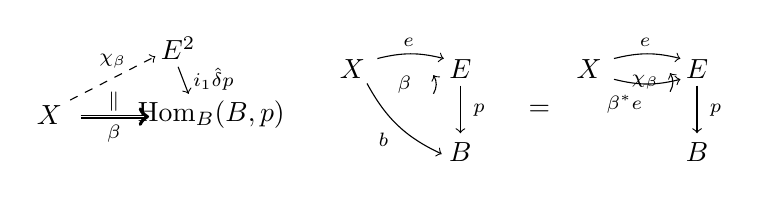
\begin{tikzpicture}[x=1.5em,y=1.5em]
  \node (E2) at (3.1,1.6) {$E^{2}$};
  \node (X)  at (0,0) {$X$};
  \node (HB) at (3.9,0) {$\mathrm{Hom}_{B}(B,p)$};
  \draw[->,dashed] (0.5,0.35) -- node[above,pos=0.5]{$\scriptstyle\qcor{\chi_{\beta}}$} (2.55,1.4);
  \draw[->] (3.1,1.15) -- (3.35,0.5);
  \node at (3.95,0.85) {$\scriptstyle i_{1}\hat{\delta}p$};
  \draw[double,->] (0.75,-0.05) -- (2.4,-0.05);
  \node at (1.55,0.32) {$\scriptstyle\parallel$};
  \node at (1.55,-0.45) {$\scriptstyle\qcor{\beta}$};
  \node at (6.1,0.7) {$\rightsquigarrow$};
  \begin{scope}[shift={(7.3,0)}]
  \node (E) at (2.6,1.1) {$E$};
  \node (X) at (0,1.1) {$X$};
  \node (B) at (2.6,-0.9) {$B$};
  \draw[->] (0.6,1.35) to[bend left=14] (2.2,1.35);
  \node at (1.35,1.75) {$\scriptstyle e$};
  \draw[->] (2.6,0.7) -- (2.6,-0.45);
  \node at (3.05,0.1) {$\scriptstyle p$};
  \draw[->] (0.35,0.75) to[bend right=18] (2.15,-0.95);
  \node at (0.75,-0.6) {$\scriptstyle b$};
  \draw[->] (1.95,0.5) to[bend right=30] (1.95,0.95);
  \node at (1.25,0.72) {$\scriptstyle\beta$};
  \node at (4.5,0.1) {$=$};
  \end{scope}
  \begin{scope}[shift={(13.0,0)}]
  \node (E) at (2.6,1.1) {$E$};
  \node (X) at (0,1.1) {$X$};
  \node (B) at (2.6,-0.9) {$B$};
  \draw[->] (0.6,1.35) to[bend left=14] (2.2,1.35);
  \node at (1.35,1.75) {$\scriptstyle e$};
  \draw[->] (0.6,0.85) to[bend right=14] (2.2,0.85);
  \node at (0.85,0.25) {$\scriptstyle\beta^{*}e$};
  \draw[->] (2.6,0.7) -- (2.6,-0.45);
  \node at (3.05,0.1) {$\scriptstyle p$};
  \draw[->] (1.95,0.55) to[bend right=30] (1.95,1.0);
  \node at (1.35,0.78) {$\scriptstyle\chi_{\beta}$};
  \end{scope}
\end{tikzpicture}
\end{center}
\end{definition}

由练习 5.1.i，提升性质究竟像上右图那样在\trHomotopyTwoCategory{}中表述，还是像
上左图那样用表示箭头来表述，并没有任何差别。

\begin{remark}\label{rem:equivalence-invariance}
\trInfinityCategory{}论的一条指导性原则是：一切\trInfinityCategory{}概念都应当
是\trEquivalence{}不变的。然而，若把 $E$ 与 $B$ 换成与之等价的%
\trInfinityCategory{} $E'$ 与 $B'$，那个与原来等价的函子 $p'\colon E\to B$
却未必是\trIsofibration。不过，由
引理 1.2.19，$p'$ 在 $B'$ 之上等价于某条\trIsofibration{} $p''$，因此我们本可以
在 $p''$ 是\cref{def:cartesian-fibration}意义下的\trIsofibration{}时，就宣布
$p'$ 为\trCartesianFibration。由推论 5.3.1，这一定义至此便是\trEquivalence{}不
变的。出于诸如命题 6.3.14 之类的技术性原因，我们更愿意让%
\cref{def:cartesian-fibration}保持其原貌。
\end{remark}

\trCartesianFibration{}的某些稳定性性质可以直接从这个定义出发来证明。

\begin{lemma}\label{lem:composite-cartesian-fibration}
若 $p\colon E\twoheadrightarrow B$ 与 $q\colon B\twoheadrightarrow A$ 都是%
\trCartesianFibration，则 $qp\colon E\twoheadrightarrow A$ 亦然。此外，%
\trNaturalTransformation
\cellpair{X}{E}{e'}{e}{\psi}
是 $qp$-\trCartesian，当且仅当 $\psi$ 是 $p$-\trCartesian{}且 $p\psi$ 是
$q$-\trCartesian。
\end{lemma}

\begin{proof}
第一条论断立即可由第二条推出：所需的提升可以先取一条 $q$-笛卡尔提升%
$\chi_{\alpha}$、再对该提升后的胞腔取 $p$-笛卡尔提升 $\chi_{\chi_{\alpha}}$ 而
构造出来。
\begin{center}
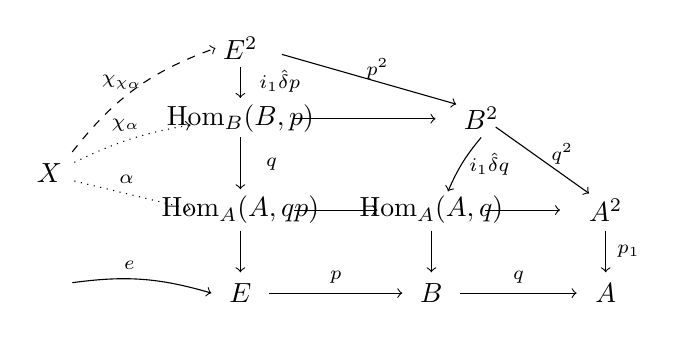
\begin{tikzpicture}[x=1.5em,y=1.5em]
  \node (E2)  at (4.6,4.3) {$E^{2}$};
  \node (HB)  at (4.6,2.6) {$\mathrm{Hom}_{B}(B,p)$};
  \node (B2)  at (10.4,2.6) {$B^{2}$};
  \node (X)   at (0,1.3) {$X$};
  \node (HA)  at (4.6,0.4) {$\mathrm{Hom}_{A}(A,qp)$};
  \node (HAq) at (9.2,0.4) {$\mathrm{Hom}_{A}(A,q)$};
  \node (A2)  at (13.4,0.4) {$A^{2}$};
  \node (E)   at (4.6,-1.6) {$E$};
  \node (B)   at (9.2,-1.6) {$B$};
  \node (A)   at (13.4,-1.6) {$A$};
  \draw[->,dashed] (0.55,1.8) to[bend left=16] node[above,pos=0.4]{$\scriptstyle\qcor{\chi_{\chi_{\alpha}}}$} (4.0,4.3);
  \draw[->] (4.6,3.85) -- (4.6,3.1);
  \node at (5.55,3.5) {$\scriptstyle i_{1}\hat{\delta}p$};
  \draw[->] (5.6,4.15) -- (9.8,2.95);
  \node at (7.9,3.8) {$\scriptstyle p^{2}$};
  \draw[->] (5.9,2.6) -- (9.3,2.6);
  \node at (6.4,2.9) {$\scriptstyle\llcorner$};
  \draw[->] (4.6,2.15) -- (4.6,0.9);
  \node at (5.35,1.5) {$\scriptstyle q$};
  \draw[->] (10.4,2.15) to[bend right=8] (9.6,0.85);
  \node at (10.6,1.5) {$\scriptstyle i_{1}\hat{\delta}q$};
  \draw[->] (10.75,2.4) -- (13.0,0.8);
  \node at (12.35,1.75) {$\scriptstyle q^{2}$};
  \draw[->,dotted] (0.6,1.55) to[bend left=8] node[above,pos=0.45]{$\scriptstyle\qcor{\chi_{\alpha}}$} (3.4,2.45);
  \draw[->,dotted] (0.6,1.1) -- node[above,pos=0.45]{$\scriptstyle\qcor{\alpha}$} (3.4,0.42);
  \draw[->] (5.9,0.4) -- (7.9,0.4);
  \node at (6.35,0.05) {$\scriptstyle\llcorner$};
  \draw[->] (10.5,0.4) -- (12.3,0.4);
  \node at (10.95,0.05) {$\scriptstyle\llcorner$};
  \draw[->] (13.4,-0.1) -- (13.4,-1.1);
  \node at (13.95,-0.6) {$\scriptstyle p_{1}$};
  \draw[->] (4.6,-0.1) -- (4.6,-1.1);
  \draw[->] (9.2,-0.1) -- (9.2,-1.1);
  \draw[->] (0.55,-1.35) to[bend left=12] node[above,pos=0.4]{$\scriptstyle e$} (3.9,-1.6);
  \draw[->] (5.3,-1.6) -- node[above]{$\scriptstyle p$} (8.5,-1.6);
  \draw[->] (9.9,-1.6) -- node[above]{$\scriptstyle q$} (12.7,-1.6);
\end{tikzpicture}
\end{center}
为证明第二条论断，先考虑一支\trNaturalTransformation{}
$\psi\colon e'\Rightarrow e$：设其为 $p$-\trCartesian，且 $p\psi$ 为
$q$-\trCartesian。由引理 5.1.2，这些性质由诸虚\trTrivialFibration{}%
表达，其中后者经拉回可定义出点线\trTrivialFibration：
\begin{center}
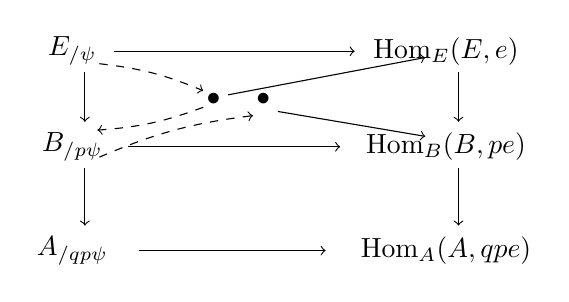
\begin{tikzpicture}[x=1.5em,y=1.5em]
  \node (Ep) at (0,4.4) {$E_{/\psi}$};
  \node (HE) at (9.0,4.4) {$\mathrm{Hom}_{E}(E,e)$};
  \node (Bp) at (0,2.1) {$B_{/p\psi}$};
  \node (HB) at (9.0,2.1) {$\mathrm{Hom}_{B}(B,pe)$};
  \node (Ap) at (0,-0.4) {$A_{/qp\psi}$};
  \node (HA) at (9.0,-0.4) {$\mathrm{Hom}_{A}(A,qpe)$};
  \draw[->] (1.0,4.4) -- (6.8,4.4);
  \draw[->] (1.35,2.1) -- (6.45,2.1);
  \draw[->] (1.6,-0.4) -- (6.1,-0.4);
  \draw[->] (0.3,3.9) -- (0.3,2.7);
  \draw[->] (9.3,3.9) -- (9.3,2.7);
  \draw[->] (0.3,1.6) -- (0.3,0.2);
  \draw[->] (9.3,1.6) -- (9.3,0.2);
  \node at (3.4,3.25) {$\bullet$};
  \node at (3.85,2.95) {$\scriptstyle\lrcorner$};
  \draw[->,dashed] (0.65,4.1) to[bend left=8] (3.15,3.45);
  \draw[->,dashed] (3.15,3.05) to[bend left=8] (0.6,2.5);
  \draw[->] (3.75,3.35) -- (8.5,4.25);
  \node at (4.6,3.25) {$\bullet$};
  \node at (5.05,2.95) {$\scriptstyle\lrcorner$};
  \draw[->,dashed] (0.65,1.85) to[bend left=8] (4.35,2.85);
  \draw[->] (4.95,2.95) -- (8.5,2.35);
\end{tikzpicture}
\end{center}
由于\trTrivialFibration{}可复合，这告诉我们
$E_{/\psi}\twoheadrightarrow A_{/qp\psi}\times_{\mathrm{Hom}_{A}(A,qpe)}\mathrm{Hom}_{E}(E,e)$
是一条\trTrivialFibration，从而 $\psi$ 是 $qp$-\trCartesian。

反之，若 $\psi$ 是 $qp$-\trCartesian，则由引理 5.1.11，它与 $qp\psi$ 的所有其余%
$qp$-笛卡尔提升同构。上面给出的构造对任何一支 $p$-笛卡尔、且在 $p$ 之下的像为%
$q$-\trCartesian 2-胞腔都产生一个 $qp$-笛卡尔提升。由引理 5.1.6 关于 $p$-与%
$q$-笛卡尔变换的同构稳定性，$\psi$ 也必具备这些性质。
\end{proof}

\begin{proposition}[拉回稳定性]\label{prop:pullback-stability}
在任何\trPullback{}方块
\begin{center}
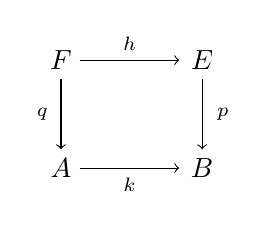
\begin{tikzpicture}[x=1.5em,y=1.5em]
  \node (F) at (0,1.3) {$F$};
  \node (E) at (3.4,1.3) {$E$};
  \node (A) at (0,-1.3) {$A$};
  \node (B) at (3.4,-1.3) {$B$};
  \draw[->] (0.45,1.3) -- node[above]{$\scriptstyle h$} (2.85,1.3);
  \draw[->] (0.45,-1.3) -- node[below]{$\scriptstyle k$} (2.85,-1.3);
  \draw[->] (0,0.85) -- (0,-0.85);
  \node at (-0.45,0) {$\scriptstyle q$};
  \draw[->] (3.4,0.85) -- (3.4,-0.85);
  \node at (3.9,0) {$\scriptstyle p$};
  \node at (0.45,0.85) {$\scriptstyle\llcorner$};
\end{tikzpicture}
\end{center}
中，若 $p$ 是一条\trCartesianFibration，则 $q$ 亦是。此外，余定义域为 $F$ 的%
\trNaturalTransformation{} $\psi$ 是 $q$-\trCartesian，当且仅当 $h\psi$ 是%
$p$-\trCartesian。
\end{proposition}

\begin{proof}
题设中的\trPullback{}方块诱导出 $i_{1}\colon 1\hookrightarrow 2$ 分别与 $q$ 和
$p$ 的\trLeibnizCotensor{}之间的一个\trPullback{}方块。考虑表示\trNaturalTransformation{}
$\alpha\colon a\Rightarrow qf$ 的一支箭头 $\qcor{\alpha}\colon X\to\mathrm{Hom}_{A}(A,q)$。
由于 $p$ 是\trCartesianFibration，\trNaturalTransformation{}
$k\alpha\colon ka\Rightarrow kqf=phf$ 容有一个 $p$-笛卡尔提升 $\qcor{\tau}$，
后者借助\trPullback{}的\trUniversalProperty{}诱导出一个提升
$\qcor{\sigma}\colon X\to F^{2}$，满足 $\qcor{h\sigma}$ 是 $p$-笛卡尔箭头：
\begin{center}
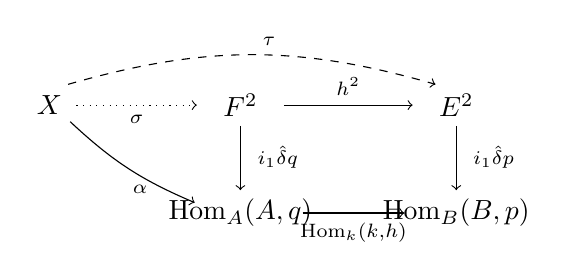
\begin{tikzpicture}[x=1.5em,y=1.5em]
  \node (X)  at (0,1.3) {$X$};
  \node (F2) at (4.6,1.3) {$F^{2}$};
  \node (E2) at (9.8,1.3) {$E^{2}$};
  \node (HA) at (4.6,-1.3) {$\mathrm{Hom}_{A}(A,q)$};
  \node (HB) at (9.8,-1.3) {$\mathrm{Hom}_{B}(B,p)$};
  \draw[->,dotted] (0.65,1.3) -- node[below]{$\scriptstyle\qcor{\sigma}$} (3.55,1.3);
  \draw[->] (5.65,1.3) -- node[above]{$\scriptstyle h^{2}$} (8.75,1.3);
  \node at (5.1,0.95) {$\scriptstyle\llcorner$};
  \draw[->] (0.5,0.9) to[bend right=10] node[below,pos=0.6]{$\scriptstyle\qcor{\alpha}$} (3.5,-1.05);
  \draw[->] (4.6,0.8) -- (4.6,-0.75);
  \node at (5.5,0.05) {$\scriptstyle i_{1}\hat{\delta}q$};
  \draw[->] (9.8,0.8) -- (9.8,-0.75);
  \node at (10.7,0.05) {$\scriptstyle i_{1}\hat{\delta}p$};
  \draw[->] (6.1,-1.3) -- node[below]{$\scriptstyle\mathrm{Hom}_{k}(k,h)$} (8.55,-1.3);
  \draw[->,dashed] (0.45,1.8) to[bend left=16] node[above,pos=0.55]{$\scriptstyle\qcor{\tau}$} (9.3,1.8);
\end{tikzpicture}
\end{center}

所以，如果我们证明了题设的第二部分——余定义域为 $F$ 的\trNaturalTransformation{}
$\psi\colon f'\Rightarrow f$ 是 $q$-\trCartesian，当且仅当 $h\psi$ 是 $p$-\trCartesian
——那么我们就证明了 $q$ 本身是一条\trCartesianFibration，其笛卡尔胞腔由%
\trPullback{}创造。

为此目的，考虑如下立方体：
\begin{center}
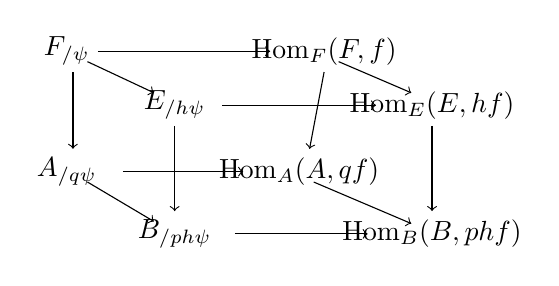
\begin{tikzpicture}[x=1.5em,y=1.5em]
  \node (Fp)  at (0,3.4) {$F_{/\psi}$};
  \node (HFf) at (6.2,3.4) {$\mathrm{Hom}_{F}(F,f)$};
  \node (Eh)  at (2.6,2.1) {$E_{/h\psi}$};
  \node (HEh) at (8.8,2.1) {$\mathrm{Hom}_{E}(E,hf)$};
  \node (Aq)  at (0,0.5) {$A_{/q\psi}$};
  \node (HAq) at (5.6,0.5) {$\mathrm{Hom}_{A}(A,qf)$};
  \node (Bph) at (2.6,-1.0) {$B_{/ph\psi}$};
  \node (HBp) at (8.8,-1.0) {$\mathrm{Hom}_{B}(B,phf)$};
  \draw[->] (0.75,3.4) -- (4.9,3.4);
  \draw[->] (3.75,2.1) -- (7.45,2.1);
  \draw[->] (1.35,0.5) -- (4.25,0.5);
  \draw[->] (4.05,-1.0) -- (7.25,-1.0);
  \draw[->] (0.15,2.9) -- (0.15,1.05);
  \draw[->] (2.6,1.6) -- (2.6,-0.45);
  \draw[->] (6.2,2.9) -- (5.85,1.05);
  \draw[->] (8.8,1.6) -- (8.8,-0.45);
  \draw[->] (0.5,3.15) -- (2.1,2.4);
  \node at (0.55,2.7) {$\scriptstyle\llcorner$};
  \draw[->] (6.55,3.15) -- (8.3,2.4);
  \draw[->] (0.5,0.25) -- (2.1,-0.7);
  \node at (0.55,-0.15) {$\scriptstyle\llcorner$};
  \draw[->] (5.95,0.25) -- (8.3,-0.75);
\end{tikzpicture}
\end{center}
由超立方体拉回引理，左面与右面都是严格的\trPullback{}方块。于是，从
$E_{/h\psi}$ 到前面中\trPullback{}的映射经拉回即得从 $F_{/\psi}$ 到后面中%
\trPullback{}的映射。从而，由命题 3.3.4，若 $h\psi$ 是 $p$-\trCartesian，则 $\psi$
是 $q$-\trCartesian。这就完成了 $q$ 是\trCartesianFibration{}的证明。

现在，若 $\psi$ 是 $q$-\trCartesian，则由引理 5.1.11，$\psi$ 与本证明第一部分中
构造的 $q\psi$ 的 $q$-笛卡尔提升 $\sigma$ 同构。于是 $h\psi$ 与 $h\sigma=\tau$
同构，后者是 $p$-\trCartesian，故由引理 5.1.6，$h\psi$ 也必是 $p$-\trCartesian。
\end{proof}

事实上，在\cref{def:cartesian-fibration}中只需假设：余定义域穿过 $p$ 的那个
泛变换容有一个 $p$-笛卡尔提升：

\begin{lemma}\label{lem:right-comma-cone-lift}
一条\trIsofibration{} $p\colon E\twoheadrightarrow B$ 是\trCartesianFibration，
当且仅当下方左图展示的 $p$ 之上的右逗号锥容有一个如下右图所示的 $p$-笛卡尔提升
$\chi$：
\begin{rveq}\label{eq:right-comma-cone}
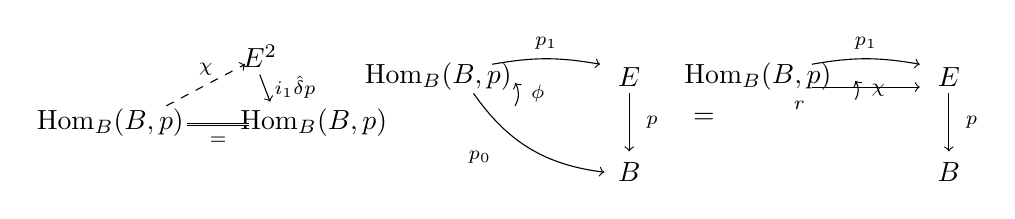
\begin{tikzpicture}[x=1.5em,y=1.5em]
  \node (E2) at (3.6,1.6) {$E^{2}$};
  \node (H1) at (0,0) {$\mathrm{Hom}_{B}(B,p)$};
  \node (H2) at (4.9,0) {$\mathrm{Hom}_{B}(B,p)$};
  \draw[->,dashed] (1.35,0.4) -- node[above,pos=0.5]{$\scriptstyle\qcor{\chi}$} (3.25,1.4);
  \draw[->] (3.6,1.15) -- (3.85,0.5);
  \node at (4.45,0.85) {$\scriptstyle i_{1}\hat{\delta}p$};
  \draw[double] (1.85,-0.05) -- (3.35,-0.05);
  \node at (2.6,-0.45) {$\scriptstyle=$};
  \node at (6.6,0.7) {$\rightsquigarrow$};
  \begin{scope}[shift={(7.9,0)}]
  \node (H) at (0,1.1) {$\mathrm{Hom}_{B}(B,p)$};
  \node (E) at (4.6,1.1) {$E$};
  \node (B) at (4.6,-1.2) {$B$};
  \draw[->] (1.3,1.4) to[bend left=10] node[above]{$\scriptstyle p_{1}$} (3.9,1.4);
  \draw[->] (4.6,0.7) -- (4.6,-0.7);
  \node at (5.15,0) {$\scriptstyle p$};
  \draw[->] (0.85,0.7) to[bend right=24] (4.0,-1.2);
  \node at (1.0,-0.85) {$\scriptstyle p_{0}$};
  \draw[->] (1.85,0.4) to[bend right=30] (1.85,0.95);
  \node at (2.4,0.68) {$\scriptstyle\phi$};
  \node at (6.4,0.1) {$=$};
  \end{scope}
  \begin{scope}[shift={(15.6,0)}]
  \node (H) at (0,1.1) {$\mathrm{Hom}_{B}(B,p)$};
  \node (E) at (4.6,1.1) {$E$};
  \node (B) at (4.6,-1.2) {$B$};
  \draw[->] (1.3,1.4) to[bend left=10] node[above]{$\scriptstyle p_{1}$} (3.9,1.4);
  \draw[->] (1.3,0.85) -- (3.9,0.85);
  \node at (1.0,0.4) {$\scriptstyle r$};
  \draw[->] (4.6,0.7) -- (4.6,-0.7);
  \node at (5.15,0) {$\scriptstyle p$};
  \draw[->] (2.35,0.55) to[bend right=30] (2.35,1.0);
  \node at (2.9,0.78) {$\scriptstyle\chi$};
  \end{scope}
\end{tikzpicture}
\end{rveq}
\end{lemma}

\begin{proof}
由定理 5.1.7(ii)，说 $p$ 之上的右逗号锥容有一个 $p$-笛卡尔提升 $\chi$，就是说%
$\qcor{\chi}$ 定义了恒同穿过 $i_{1}\hat{\delta}p$ 的一个绝对右提升。由引理
2.3.6 即知，限制
\begin{center}
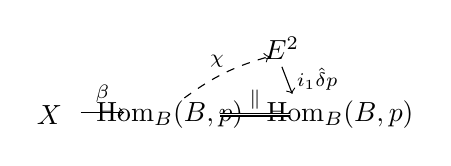
\begin{tikzpicture}[x=1.5em,y=1.5em]
  \node (E2) at (5.6,1.6) {$E^{2}$};
  \node (X)  at (0,0) {$X$};
  \node (H1) at (2.9,0) {$\mathrm{Hom}_{B}(B,p)$};
  \node (H2) at (7.0,0) {$\mathrm{Hom}_{B}(B,p)$};
  \draw[->] (0.75,0.05) -- node[above]{$\scriptstyle\qcor{\beta}$} (1.8,0.05);
  \draw[double] (4.1,0) -- (5.8,0);
  \node at (4.95,0.35) {$\scriptstyle\parallel$};
  \draw[->,dashed] (3.25,0.4) to[bend left=10] node[above,pos=0.4]{$\scriptstyle\qcor{\chi}$} (5.3,1.4);
  \draw[->] (5.6,1.15) -- (5.85,0.5);
  \node at (6.45,0.85) {$\scriptstyle i_{1}\hat{\delta}p$};
\end{tikzpicture}
\end{center}
对任意 $\qcor{\beta}\colon X\to\mathrm{Hom}_{B}(B,p)$ 都定义了一个绝对右提升，
从而由定理 5.1.7(ii)，任何 $\beta\colon b\Rightarrow pe$ 都容有一个 $p$-笛卡尔
提升。
\end{proof}

当 $p$ 是\trCartesianFibration{}时，我们把 \eqref{eq:right-comma-cone} 的泛%
笛卡尔箭头 $\qcor{\chi}\colon\mathrm{Hom}_{B}(B,p)\to E^{2}$ 称作%
\textbf{泛 $p$-笛卡尔提升}（generic $p$-cartesian lift）。

\begin{remark}[笛卡尔纤维化的纤维上的箭头作用]\label{rem:fiber-action}
\trCartesianFibration{}的底范畴中一支箭头在诸\trFiber{}上的作用可以描述如下。
考虑余定义域为 $B$ 的\trNaturalTransformation{} $\beta$，并作出 $p$ 在其定义域
函子与余定义域函子之上的诸\trFiber
\begin{center}
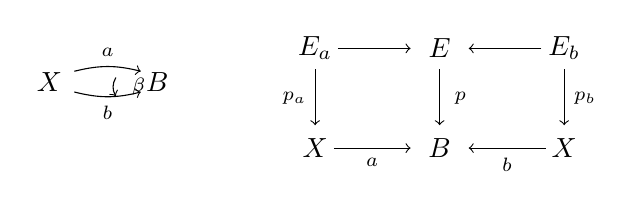
\begin{tikzpicture}[x=1.5em,y=1.5em]
  \begin{scope}[shift={(0,0.5)}]
  \node (B) at (2.6,0) {$B$};
  \node (X) at (0,0) {$X$};
  \draw[->] (0.6,0.25) to[bend left=14] node[above]{$\scriptstyle a$} (2.2,0.25);
  \draw[->] (0.6,-0.25) to[bend right=14] node[below]{$\scriptstyle b$} (2.2,-0.25);
  \draw[->] (1.6,0.1) to[bend right=30] (1.6,-0.35);
  \node at (2.15,-0.12) {$\scriptstyle\beta$};
  \end{scope}
  \begin{scope}[shift={(6.4,0)}]
  \node (Ea) at (0,1.3) {$E_{a}$};
  \node (E)  at (3.0,1.3) {$E$};
  \node (Eb) at (6.0,1.3) {$E_{b}$};
  \node (Xa) at (0,-1.1) {$X$};
  \node (Bm) at (3.0,-1.1) {$B$};
  \node (Xb) at (6.0,-1.1) {$X$};
  \draw[->] (0.55,1.3) -- (2.3,1.3);
  \draw[->] (5.45,1.3) -- (3.7,1.3);
  \draw[->] (0,0.8) -- (0,-0.55);
  \node at (-0.5,0.1) {$\scriptstyle p_{a}$};
  \draw[->] (3.0,0.8) -- (3.0,-0.55);
  \node at (3.5,0.1) {$\scriptstyle p$};
  \draw[->] (6.0,0.8) -- (6.0,-0.55);
  \node at (6.5,0.1) {$\scriptstyle p_{b}$};
  \draw[->] (0.45,-1.1) -- node[below]{$\scriptstyle a$} (2.3,-1.1);
  \draw[->] (5.55,-1.1) -- node[below]{$\scriptstyle b$} (3.7,-1.1);
  \node at (0.42,0.72) {$\scriptstyle\llcorner$};
  \node at (5.58,0.72) {$\scriptstyle\lrcorner$};
  \end{scope}
\end{tikzpicture}
\end{center}
定义\trFiber{} $E_{b}$ 的\trPullback{}方块可以像下左那样分解
\begin{center}
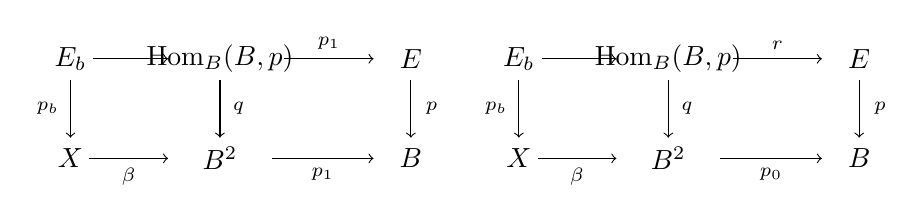
\begin{tikzpicture}[x=1.5em,y=1.5em]
  \begin{scope}[shift={(0,0)}]
  \node (Eb) at (0,1.4) {$E_{b}$};
  \node (H)  at (3.6,1.4) {$\mathrm{Hom}_{B}(B,p)$};
  \node (E)  at (8.2,1.4) {$E$};
  \node (X)  at (0,-1.0) {$X$};
  \node (B2) at (3.6,-1.0) {$B^{2}$};
  \node (B)  at (8.2,-1.0) {$B$};
  \draw[->] (0.55,1.4) -- (2.35,1.4);
  \draw[->] (5.15,1.4) -- node[above]{$\scriptstyle p_{1}$} (7.3,1.4);
  \draw[->] (0,0.9) -- (0,-0.5);
  \node at (-0.55,0.2) {$\scriptstyle p_{b}$};
  \draw[->] (3.6,0.9) -- (3.6,-0.5);
  \node at (4.05,0.2) {$\scriptstyle q$};
  \draw[->] (8.2,0.9) -- (8.2,-0.5);
  \node at (8.7,0.2) {$\scriptstyle p$};
  \draw[->] (0.45,-1.0) -- node[below]{$\scriptstyle\qcor{\beta}$} (2.35,-1.0);
  \draw[->] (4.85,-1.0) -- node[below]{$\scriptstyle p_{1}$} (7.3,-1.0);
  \node at (0.45,0.85) {$\scriptstyle\llcorner$};
  \node at (5.2,0.85) {$\scriptstyle\llcorner$};
  \end{scope}
  \begin{scope}[shift={(10.8,0)}]
  \node (Eb) at (0,1.4) {$E_{b}$};
  \node (H)  at (3.6,1.4) {$\mathrm{Hom}_{B}(B,p)$};
  \node (E)  at (8.2,1.4) {$E$};
  \node (X)  at (0,-1.0) {$X$};
  \node (B2) at (3.6,-1.0) {$B^{2}$};
  \node (B)  at (8.2,-1.0) {$B$};
  \draw[->] (0.55,1.4) -- (2.35,1.4);
  \draw[->] (5.15,1.4) -- node[above]{$\scriptstyle r$} (7.3,1.4);
  \draw[->] (0,0.9) -- (0,-0.5);
  \node at (-0.55,0.2) {$\scriptstyle p_{b}$};
  \draw[->] (3.6,0.9) -- (3.6,-0.5);
  \node at (4.05,0.2) {$\scriptstyle q$};
  \draw[->] (8.2,0.9) -- (8.2,-0.5);
  \node at (8.7,0.2) {$\scriptstyle p$};
  \draw[->] (0.45,-1.0) -- node[below]{$\scriptstyle\qcor{\beta}$} (2.35,-1.0);
  \draw[->] (4.85,-1.0) -- node[below]{$\scriptstyle p_{0}$} (7.3,-1.0);
  \node at (0.45,0.85) {$\scriptstyle\llcorner$};
  \end{scope}
\end{tikzpicture}
\end{center}
从而上右展示的矩形在定义 $E_{a}$ 的那个\trPullback{}之上定义了一个\trCone，诱导出
映射 $\beta^{*}\colon E_{b}\to E_{a}$。此矩形中顶部的水平函子复原了余定义域为
$\ell_{b}$ 的 $\beta$ 的 $p$-笛卡尔提升的定义域分量 $\beta^{*}(\ell_{b})$。这与
(5.0.1) 中给出的 $\beta^{*}\colon E_{b}\to E_{a}$ 的描述相吻合。
\end{remark}

\cref{lem:right-comma-cone-lift}可以加以扩充，给出\trCartesianFibration{}%
的一个内部刻画，其灵感来自 Street [118, 119, 121] 的一条类似结果，而后者又受
Gray [48] 论及他所称「Chevalley 判据」\footnote{Gray 把 [48, 3.11]——即%
\cref{thm:internal-characterization}的 $(i)\Leftrightarrow(ii)$ 等价在%
\trInfinityCosmos{} $\mathcal{C}at$ 中的特例——归功于 Claude Chevalley 1962 年
在 Berkeley 开设的一个讨论班的未发表讲义。}的先前工作所启发（另见 [131]）。我们
将会看到，\trCartesianFibration{}
$p\colon E\twoheadrightarrow B$ 的\trUniversalProperty{}可以由如下数据编码：由
恒同 2-胞腔诱导出的函子 $\Delta_{p}\colon E\to\mathrm{Hom}_{B}(B,p)$ 的某个合适
的\trRightAdjoint，或者把 $p$ 应用于余定义域为 $E$ 的\trGenericArrow{}而定义的
函子 $i_{1}\hat{\delta}p\colon E^{2}\to\mathrm{Hom}_{B}(B,p)$ 的某个合适的%
\trRightAdjoint。事实上，只要把定理 5.1.7 中 $p$-笛卡尔胞腔的诸刻画特化到%
\cref{lem:right-comma-cone-lift}所描述的泛情形，这条结果就相当容易地随之得出。

\begin{theorem}[笛卡尔纤维化的一个内部刻画]\label{thm:internal-characterization}
对一条\trIsofibration{} $p\colon E\twoheadrightarrow B$，下列诸条等价：
\begin{enumerate}[label=(\roman*)]
\item $p\colon E\twoheadrightarrow B$ 定义了一条\trCartesianFibration。
\item 函子 $i_{1}\hat{\delta}p\colon E^{2}\to\mathrm{Hom}_{B}(B,p)$
容有一个右伴随右逆：%
\footnote{由引理 3.6.9，这样的伴随可以矫正为在 $\mathrm{Hom}_{B}(B,p)$
之上纤维化的伴随；故 $\qcor{\chi}\colon\mathrm{Hom}_{B}(B,p)\to E^{2}$
可解释为「$E^{2}$ 在 $\mathrm{Hom}_{B}(B,p)$ 之上由 $\qcor{\chi}$
切出的一个\trTerminal{}\trElement{}」（见定义 3.6.8）。}
\begin{center}
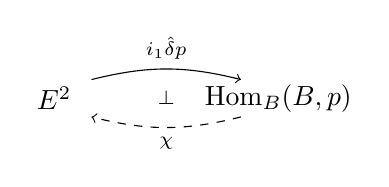
\begin{tikzpicture}[x=1.5em,y=1.5em]
  \node (E2) at (0,0) {$E^{2}$};
  \node (H)  at (5.4,0) {$\mathrm{Hom}_{B}(B,p)$};
  \draw[->] (0.9,0.45) to[bend left=14] node[above]{$\scriptstyle i_{1}\hat{\delta}p$} (4.5,0.45);
  \node at (2.7,0) {$\scriptstyle\perp$};
  \draw[->,dashed] (4.5,-0.45) to[bend left=14] node[below]{$\scriptstyle\qcor{\chi}$} (0.9,-0.45);
\end{tikzpicture}
\end{center}
\item 函子 $\Delta_{p}\colon E\to\mathrm{Hom}_{B}(B,p)$ 容有一个 $B$ 上的%
\trRightAdjoint：\footnote{由引理 3.5.9，$\Delta_{p}\simeq\qcor{\mathrm{id}_{p}}$
本身就是余定义域投影函子 $p_{1}\colon\mathrm{Hom}_{B}(B,p)\to E$ 在 $E$ 之上、
从而也在 $B$ 之上的\trRightAdjoint。由于伴随 $p_{1}\dashv\Delta_{p}$ 的%
\trCounit{}是一个\trIsomorphism，故只要 (iii) 中所假设的伴随存在（见引理
B.3.9），形式上即可推出伴随 $\Delta_{p}\dashv r$ 的\trUnit{}也必是%
\trIsomorphism。于是 $r$ 定义了 $\Delta_{p}$ 在 $B$ 之上的一个右伴随左逆。}
\begin{center}
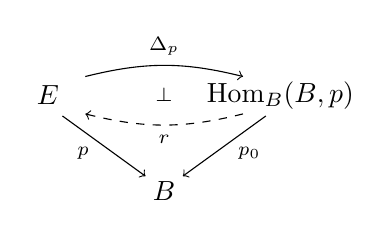
\begin{tikzpicture}[x=1.5em,y=1.5em]
  \node (E) at (0,0) {$E$};
  \node (H) at (5.6,0) {$\mathrm{Hom}_{B}(B,p)$};
  \draw[->] (0.9,0.45) to[bend left=14] node[above]{$\scriptstyle\Delta_{p}$} (4.7,0.45);
  \node at (2.8,0) {$\scriptstyle\perp$};
  \draw[->,dashed] (4.7,-0.45) to[bend left=14] node[below]{$\scriptstyle r$} (0.9,-0.45);
  \node (B) at (2.8,-2.3) {$B$};
  \draw[->] (0.35,-0.5) -- (2.35,-1.95);
  \node at (0.85,-1.4) {$\scriptstyle p$};
  \draw[->] (5.25,-0.5) -- (3.25,-1.95);
  \node at (4.85,-1.4) {$\scriptstyle p_{0}$};
\end{tikzpicture}
\end{center}
\end{enumerate}
\end{theorem}

正如证明所揭示的，(iii) 的\trRightAdjoint{}是 \eqref{eq:right-comma-cone} 的泛%
$p$-笛卡尔提升 $\chi$ 的定义域分量，而 $\chi$ 可复原为 $p_{1}\epsilon$，其中
$\epsilon$ 是\trFiberedAdjunction{} $\Delta_{p}\dashv r$ 的\trCounit。由\trOneCellInduction，
泛笛卡尔提升 $\chi$ 可以由一个函子 $\qcor{\chi}\colon\mathrm{Hom}_{B}(B,p)\to E^{2}$
表示，而这便定义了 (ii) 的\trRightAdjoint。

\begin{proof}
我们证明 $(i)\Leftrightarrow(ii)$ 与 $(i)\Leftrightarrow(iii)$。

\textbf{(i)$\Leftrightarrow$(ii)：}由定理 5.1.7(ii) 与%
\cref{lem:right-comma-cone-lift}，
$p\colon E\twoheadrightarrow B$ 是\trCartesianFibration，当且仅当
$i_{1}\hat{\delta}p\colon E^{2}\to\mathrm{Hom}_{B}(B,p)$ 容有一个定义出绝对右
提升图的\trSection：
\begin{center}
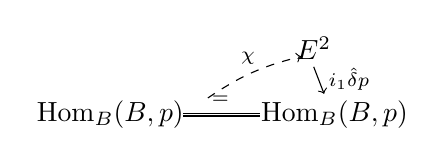
\begin{tikzpicture}[x=1.5em,y=1.5em]
  \node (E2) at (4.9,1.6) {$E^{2}$};
  \node (H1) at (0,0) {$\mathrm{Hom}_{B}(B,p)$};
  \node (H2) at (5.4,0) {$\mathrm{Hom}_{B}(B,p)$};
  \draw[double] (1.75,0) -- (3.6,0);
  \node at (2.65,0.35) {$\scriptstyle=$};
  \draw[->,dashed] (2.35,0.4) to[bend left=10] node[above,pos=0.45]{$\scriptstyle\qcor{\chi}$} (4.6,1.4);
  \draw[->] (4.9,1.15) -- (5.15,0.5);
  \node at (5.75,0.85) {$\scriptstyle i_{1}\hat{\delta}p$};
\end{tikzpicture}
\end{center}
由引理 2.3.7，这样的绝对右提升定义了一个余单位为恒同的伴随
$i_{1}\hat{\delta}p\dashv\qcor{\chi}$。反之，若 $i_{1}\hat{\delta}p\dashv\qcor{\chi}$
带有可逆余单位，则由于左伴随是一条\trIsofibration，它可以被矫正为一个纤维化
伴随，其中 $\qcor{\chi}$ 定义了一个严格\trSection{}而余单位是恒同。由引理
2.3.7，$\qcor{\chi}$ 于是定义了恒同函子穿过 $i_{1}\hat{\delta}p$ 的一个绝对右
提升，这就证明 $p$ 是一条\trCartesianFibration。

\textbf{(i)$\Leftrightarrow$(iii)：}若 $p\colon E\twoheadrightarrow B$ 是%
\trInfinityCosmos{} $\mathcal{K}$中的一条\trCartesianFibration，则由定理
5.1.7(iii) 存在绝对右提升图表
\begin{center}
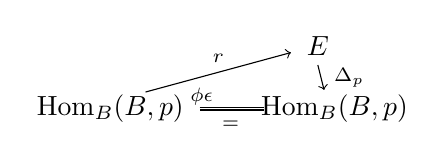
\begin{tikzpicture}[x=1.5em,y=1.5em]
  \node (E)  at (5.0,1.5) {$E$};
  \node (H1) at (0,0) {$\mathrm{Hom}_{B}(B,p)$};
  \node (H2) at (5.4,0) {$\mathrm{Hom}_{B}(B,p)$};
  \draw[->] (0.85,0.4) -- node[above,pos=0.5]{$\scriptstyle r$} (4.35,1.35);
  \node at (2.2,0.3) {$\scriptstyle\phi\epsilon$};
  \draw[->] (5.0,1.05) -- (5.15,0.45);
  \node at (5.75,0.75) {$\scriptstyle\Delta_{p}$};
  \draw[double] (2.15,0) -- (3.7,0);
  \node at (2.9,-0.38) {$\scriptstyle=$};
\end{tikzpicture}
\end{center}
满足 $p_{0}\epsilon=\mathrm{id}_{p_{0}}$。由命题 3.6.2，我们可以把 $\epsilon$
提升为\trSliceInfinityCosmos{} $\mathcal{K}_{/B}$ 中的一个%
\trNaturalTransformation。在
$\mathcal{K}_{/B}$ 中应用引理 2.3.7，可见 $r$ 定义了 $\Delta_{p}$ 的一个纤维化%
\trRightAdjoint。反之，若给定一个 $B$ 上的\trFiberedAdjunction，我们可以应用遗忘 2-函子
$\hbar(\mathcal{K}_{/B})\to\hbar\mathcal{K}$ 得到一个伴随\footnote{回忆非例
1.3.6：遗忘函子 $\mathcal{K}_{/B}\to\mathcal{K}$ 不是宇宙论的。尽管如此，%
\trInfinityCosmos{}之间的任何\trSimplicialFunctor{}都会下降为其%
\trHomotopyTwoCategory{}之间
的一个\trTwoFunctor，而这正是此处所需的全部。}
\begin{center}
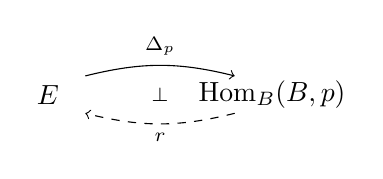
\begin{tikzpicture}[x=1.5em,y=1.5em]
  \node (E) at (0,0) {$E$};
  \node (H) at (5.4,0) {$\mathrm{Hom}_{B}(B,p)$};
  \draw[->] (0.9,0.45) to[bend left=14] node[above]{$\scriptstyle\Delta_{p}$} (4.5,0.45);
  \node at (2.7,0) {$\scriptstyle\perp$};
  \draw[->,dashed] (4.5,-0.45) to[bend left=14] node[below]{$\scriptstyle r$} (0.9,-0.45);
\end{tikzpicture}
\end{center}
然后再应用引理 2.3.7 得出：\trCounit{} $\epsilon$ 定义了恒同穿过 $\Delta_{p}$ 的
一个绝对右提升。由于余单位在「遗忘伴随在 $B$ 之上纤维化」这一过程中保持不变，
我们仍有 $p_{0}\epsilon=\mathrm{id}_{p_{0}}$，正如所需。
\end{proof}

\trCartesianFibration{}的例子早就该登场了。

\begin{proposition}[定义域投影纤维化]\label{prop:domain-projection-fibration}
对任意\trInfinityCategory{} $A$，定义域投影函子
$p_{0}\colon A^{2}\twoheadrightarrow A$ 定义了
一条\trCartesianFibration。此外，余定义域为 $A^{2}$ 的\trNaturalTransformation{}
$\psi$ 是 $p_{0}$-\trCartesian，当且仅当 $p_{1}\psi$ 可逆。
\end{proposition}

在给出证明之前，我们先解释其想法。\trNaturalTransformation
\begin{center}
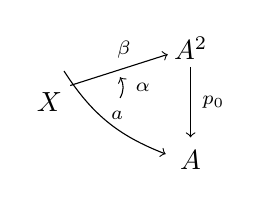
\begin{tikzpicture}[x=1.5em,y=1.5em]
  \node (A2) at (3.4,1.3) {$A^{2}$};
  \node (X)  at (0,0) {$X$};
  \node (A)  at (3.4,-1.4) {$A$};
  \draw[->] (0.5,0.4) -- node[above,pos=0.55]{$\scriptstyle\qcor{\beta}$} (2.85,1.15);
  \draw[->] (3.4,0.85) -- (3.4,-0.85);
  \node at (3.95,0) {$\scriptstyle p_{0}$};
  \draw[->] (0.35,0.75) to[bend right=18] node[above,pos=0.6]{$\scriptstyle a$} (2.8,-1.25);
  \draw[->] (1.7,0.1) to[bend right=30] (1.7,0.6);
  \node at (2.25,0.35) {$\scriptstyle\alpha$};
\end{tikzpicture}
\end{center}
定义了 $\mathrm{hFun}(X,A)$ 中一对可复合的 2-胞腔 $\alpha\colon a\Rightarrow x$
与 $\beta\colon x\Rightarrow y$。复合二者即诱导出一个 2-胞腔
\cellpair{X}{A^{2}}{\qcor{\beta\circ\alpha}}{\qcor{\beta}}{\psi}
它表示 $\mathrm{hFun}(X,A)$ 中的交换方块
\begin{center}
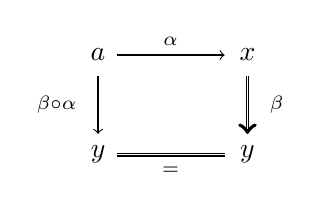
\begin{tikzpicture}[x=1.5em,y=1.5em]
  \node (a)  at (0,1.2) {$a$};
  \node (x)  at (3.6,1.2) {$x$};
  \node (y1) at (0,-1.2) {$y$};
  \node (y2) at (3.6,-1.2) {$y$};
  \draw[->] (0.45,1.2) -- node[above]{$\scriptstyle\alpha$} (3.05,1.2);
  \draw[->] (0,0.7) -- (0,-0.7);
  \node at (-1.0,0) {$\scriptstyle\beta\circ\alpha$};
  \draw[double,->] (3.6,0.7) -- (3.6,-0.7);
  \node at (4.3,0) {$\scriptstyle\beta$};
  \draw[double] (0.45,-1.2) -- (3.05,-1.2);
  \node at (1.75,-1.6) {$\scriptstyle=$};
\end{tikzpicture}
\end{center}
使得 $p_{0}\psi=\alpha$（正如所需）且 $p_{1}\psi=\mathrm{id}$。

\begin{proof}
我们使用\cref{thm:internal-characterization}(ii)，通过为函子
\begin{center}
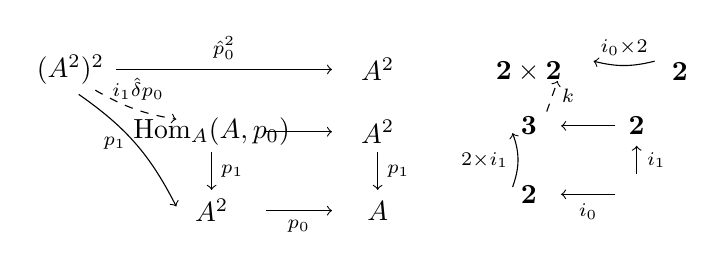
\begin{tikzpicture}[x=1.5em,y=1.5em]
  \begin{scope}[shift={(0,0)}]
  \node (A22) at (0,2.4) {$(A^{2})^{2}$};
  \node (A2t) at (7.4,2.4) {$A^{2}$};
  \node (H)   at (3.4,0.9) {$\mathrm{Hom}_{A}(A,p_{0})$};
  \node (A2m) at (7.4,0.9) {$A^{2}$};
  \node (A2b) at (3.4,-1.0) {$A^{2}$};
  \node (A)   at (7.4,-1.0) {$A$};
  \draw[->] (1.1,2.4) -- node[above]{$\scriptstyle\hat{p}_{0}^{2}$} (6.3,2.4);
  \draw[->,dashed] (0.6,1.9) to[bend right=10] node[above,pos=0.55]{$\scriptstyle i_{1}\hat{\delta}p_{0}$} (2.55,1.2);
  \draw[->] (4.7,0.9) -- (6.3,0.9);
  \node at (5.15,1.2) {$\scriptstyle\llcorner$};
  \draw[->] (0.2,1.8) to[bend left=14] node[left,pos=0.5]{$\scriptstyle p_{1}$} (2.55,-0.9);
  \draw[->] (3.4,0.4) -- (3.4,-0.5);
  \node at (3.9,-0.05) {$\scriptstyle p_{1}$};
  \draw[->] (7.4,0.4) -- (7.4,-0.5);
  \node at (7.9,-0.05) {$\scriptstyle p_{1}$};
  \draw[->] (4.7,-1.0) -- node[below]{$\scriptstyle p_{0}$} (6.3,-1.0);
  \end{scope}
  \begin{scope}[shift={(10.0,0)},x=1.3em,y=1.3em]
  \node (tt)  at (1.2,2.7) {$\qcTwo\times\qcTwo$};
  \node (t2a) at (5.4,2.7) {$\qcTwo$};
  \node (t3)  at (1.2,1.2) {$\qcThree$};
  \node (t2b) at (4.2,1.2) {$\qcTwo$};
  \node (t2c) at (1.2,-0.7) {$\qcTwo$};
  \node (t1)  at (4.2,-0.7) {$\qcOne$};
  \draw[->] (4.7,3.0) to[bend left=14] node[above,pos=0.5]{$\scriptstyle i_{0}\times 2$} (3.0,3.0);
  \draw[->,dashed] (1.7,1.6) -- node[right,pos=0.5]{$\scriptstyle k$} (2.0,2.45);
  \draw[->] (3.6,1.2) -- (2.1,1.2);
  \draw[->] (0.75,-0.5) to[bend right=20] node[left,pos=0.5]{$\scriptstyle 2\times i_{1}$} (0.75,1.0);
  \draw[->] (4.2,-0.15) -- (4.2,0.65);
  \node at (4.75,0.25) {$\scriptstyle i_{1}$};
  \draw[->] (3.6,-0.7) -- node[below]{$\scriptstyle i_{0}$} (2.1,-0.7);
  \end{scope}
\end{tikzpicture}
\end{center}
构造一个合适的伴随来证明 $p_{0}$ 是\trCartesian，该函子由与右上所展示的诸 1-范畴作%
\trCotensor{}而定义。\footnote{\trCotensor{} $A^{(-)}$ 把\trSimplicialSet{}的%
\trPushout{}送到\trInfinityCategory{}的\trPullback，而\trSimplicialSet{}
$2\sqcup_{0}2$ 的\trPushout{}是 $\wedge=\Lambda^{1}[2]$，而非
$3=\Delta[2]$。然而，由于\trInfinityCategory{}之间的\trEquivalence{}
$A^{3}\simeq A^{\wedge}$，作此处所指的替换并无妨碍。}

要为映射 $i_{1}\hat{\delta}p_{0}$ 构造一个右伴随右逆，只需为 1-范畴的包含
$k\colon\qcThree\hookrightarrow\qcTwo\times\qcTwo$——其像为
$(0,0)\to(0,1)\to(1,1)$——构造一个左伴随左逆。左伴随
$\ell\colon\qcTwo\times\qcTwo\to\qcThree$ 在 $\qcThree$ 的像上是左逆，并把
$(1,0)$ 送到 $\qcThree$ 的\trTerminal{}元素：
\[
\qcTwo\times\qcTwo\ni
\left\{\begin{array}{ccc}
(0,0) & \longrightarrow & (0,1)\\
\downarrow & & \downarrow\\
(1,0) & \longrightarrow & (1,1)
\end{array}\right\}
\;\overset{\ell}{\longmapsto}\;
\left\{\begin{array}{ccc}
0 & \longrightarrow & 1\\
\downarrow & & \downarrow\\
2 & = & 2
\end{array}\right\}
\in\qcThree
\]
现在
\begin{center}
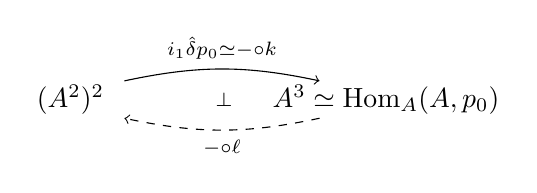
\begin{tikzpicture}[x=1.5em,y=1.5em]
  \node (A22) at (0,0) {$(A^{2})^{2}$};
  \node (A3)  at (7.6,0) {$A^{3}\simeq\mathrm{Hom}_{A}(A,p_{0})$};
  \draw[->] (1.3,0.45) to[bend left=12] node[above]{$\scriptstyle i_{1}\hat{\delta}p_{0}\simeq-\circ k$} (6.0,0.45);
  \node at (3.7,0) {$\scriptstyle\perp$};
  \draw[->,dashed] (6.0,-0.45) to[bend left=12] node[below]{$\scriptstyle-\circ\ell$} (1.3,-0.45);
\end{tikzpicture}
\end{center}
定义了所求的右伴随右逆。

$p_{0}$-笛卡尔变换的刻画由定理 5.1.7(ii) 得出。对任意箭头
$\qcor{\psi}\colon X\to A^{2}$，左下的交换三角形穿过由该伴随定义的绝对提升图
分解，而 $\qcor{\psi}$ 是 $p_{0}$-\trCartesian，当且仅当诱导出的%
\trNaturalTransformation{} $\zeta$ 可逆。
\begin{center}
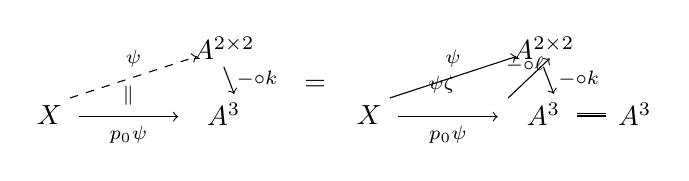
\begin{tikzpicture}[x=1.5em,y=1.5em]
  \begin{scope}[shift={(0,0)}]
  \node (A22) at (4.2,1.6) {$A^{2\times 2}$};
  \node (X)   at (0,0) {$X$};
  \node (A3)  at (4.2,0) {$A^{3}$};
  \draw[->,dashed] (0.5,0.4) -- node[above,pos=0.5]{$\scriptstyle\qcor{\psi}$} (3.55,1.4);
  \node at (1.9,0.45) {$\scriptstyle\parallel$};
  \draw[->] (0.7,-0.05) -- node[below]{$\scriptstyle\qcor{p_{0}\psi}$} (3.1,-0.05);
  \draw[->] (4.2,1.15) -- (4.45,0.5);
  \node at (5.0,0.85) {$\scriptstyle-\circ k$};
  \node at (6.4,0.7) {$=$};
  \end{scope}
  \begin{scope}[shift={(7.7,0)}]
  \node (A22) at (4.2,1.6) {$A^{2\times 2}$};
  \node (X)   at (0,0) {$X$};
  \node (A3)  at (4.2,0) {$A^{3}$};
  \node (A3b) at (6.4,0) {$A^{3}$};
  \draw[->] (0.5,0.4) -- node[above,pos=0.5]{$\scriptstyle\qcor{\psi}$} (3.55,1.4);
  \node at (1.75,0.72) {$\scriptstyle\psi\zeta$};
  \draw[->] (0.7,-0.05) -- node[below]{$\scriptstyle\qcor{p_{0}\psi}$} (3.1,-0.05);
  \draw[->] (3.35,0.4) -- node[above,pos=0.4]{$\scriptstyle-\circ\ell$} (4.35,1.35);
  \draw[double] (5.0,0) -- (5.7,0);
  \draw[->] (4.2,1.15) -- (4.45,0.5);
  \node at (5.05,0.85) {$\scriptstyle-\circ k$};
  \end{scope}
\end{tikzpicture}
\end{center}
若 $\zeta$ 是一个\trIsomorphism，则 $\qcor{\psi}$ 与沿 $\ell$ 取限制所得像中的
一支箭头同构，于是其余定义域分量必可逆。反之，若 $p_{1}\psi$ 可逆，则由定理
5.1.7(ii)，欲证 $\psi$ 是 $p_{0}$-\trCartesian，只需证 $\zeta$ 是\trIsomorphism。
由\trTwoCellConservativity{}的两次应用，只需证：以 $\qcTwo\times\qcTwo$ 的每个
元素为指标的 $\zeta$ 的四个分量都可逆。由于 $\zeta$ 沿 $k$ 限制为恒同，这些分量
中有三个必为恒同，而第四个分量
\begin{center}
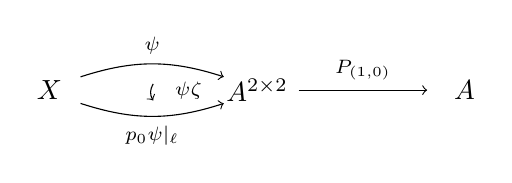
\begin{tikzpicture}[x=1.5em,y=1.5em]
  \node (X)   at (0,0) {$X$};
  \node (A22) at (5.0,0) {$A^{2\times 2}$};
  \node (A)   at (10.0,0) {$A$};
  \draw[->] (0.75,0.32) to[bend left=18] node[above]{$\scriptstyle\qcor{\psi}$} (4.2,0.32);
  \draw[->] (0.75,-0.32) to[bend right=18] node[below]{$\scriptstyle\qcor{p_{0}\psi}\vert_{\ell}$} (4.2,-0.32);
  \draw[->] (2.5,0.15) to[bend right=32] (2.5,-0.25);
  \node at (3.35,-0.02) {$\scriptstyle\psi\zeta$};
  \draw[->] (6.0,0) -- node[above]{$\scriptstyle P_{(1,0)}$} (9.1,0);
\end{tikzpicture}
\end{center}
在 $\mathrm{hFun}(X,A)$ 中等于 $p_{1}\psi$。
\end{proof}

对容许\trPullback{}的\trInfinityCategory（见定义 4.3.8），余定义域投影函子也
定义了一条\trCartesianFibration：

\begin{proposition}[余定义域投影纤维化]\label{prop:codomain-projection-fibration}
设 $A$ 是容许\trPullback{}的\trInfinityCategory。则余定义域投影函子
$p_{1}\colon A^{2}\twoheadrightarrow A$ 是一条\trCartesianFibration，且诸
$p_{1}$-笛卡尔箭头
恰是\trPullback{}方块。
\end{proposition}

\begin{proof}
我们经由\cref{thm:internal-characterization}(ii)，为函子 $i_{1}\hat{\delta}p_{1}$
寻找一个右伴随右逆，该函子由下左定义，即把 $A^{(-)}$ 应用于下右所展示的单纯集
图表：\footnote{原书此边印作 $p_{0}$，依 $\mathrm{Hom}_{A}(A,p_{1})$ 之拉回刻画
当作 $p_{1}$，径改。——译者注}
\begin{center}
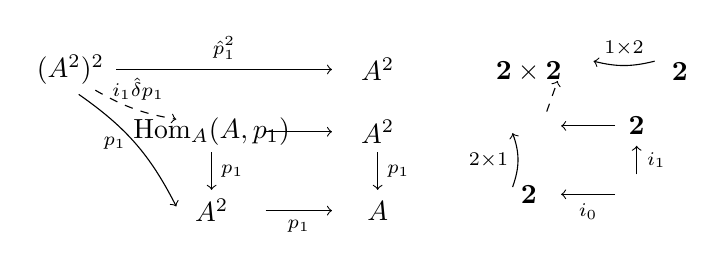
\begin{tikzpicture}[x=1.5em,y=1.5em]
  \begin{scope}[shift={(0,0)}]
  \node (A22) at (0,2.4) {$(A^{2})^{2}$};
  \node (A2t) at (7.4,2.4) {$A^{2}$};
  \node (H)   at (3.4,0.9) {$\mathrm{Hom}_{A}(A,p_{1})$};
  \node (A2m) at (7.4,0.9) {$A^{2}$};
  \node (A2b) at (3.4,-1.0) {$A^{2}$};
  \node (A)   at (7.4,-1.0) {$A$};
  \draw[->] (1.1,2.4) -- node[above]{$\scriptstyle\hat{p}_{1}^{2}$} (6.3,2.4);
  \draw[->,dashed] (0.6,1.9) to[bend right=10] node[above,pos=0.55]{$\scriptstyle i_{1}\hat{\delta}p_{1}$} (2.55,1.2);
  \draw[->] (4.7,0.9) -- (6.3,0.9);
  \node at (5.15,1.2) {$\scriptstyle\llcorner$};
  \draw[->] (0.2,1.8) to[bend left=14] node[left,pos=0.5]{$\scriptstyle p_{1}$} (2.55,-0.9);
  \draw[->] (3.4,0.4) -- (3.4,-0.5);
  \node at (3.9,-0.05) {$\scriptstyle p_{1}$};
  \draw[->] (7.4,0.4) -- (7.4,-0.5);
  \node at (7.9,-0.05) {$\scriptstyle p_{1}$};
  \draw[->] (4.7,-1.0) -- node[below]{$\scriptstyle p_{1}$} (6.3,-1.0);
  \end{scope}
  \begin{scope}[shift={(10.0,0)},x=1.3em,y=1.3em]
  \node (tt)  at (1.2,2.7) {$\qcTwo\times\qcTwo$};
  \node (t2a) at (5.4,2.7) {$\qcTwo$};
  \node (lc)  at (1.2,1.2) {$\lrcorner$};
  \node (t2b) at (4.2,1.2) {$\qcTwo$};
  \node (t2c) at (1.2,-0.7) {$\qcTwo$};
  \node (t1)  at (4.2,-0.7) {$\qcOne$};
  \draw[->] (4.7,3.0) to[bend left=14] node[above,pos=0.5]{$\scriptstyle 1\times 2$} (3.0,3.0);
  \draw[->,dashed] (1.7,1.6) -- (2.0,2.45);
  \draw[->] (3.6,1.2) -- (2.1,1.2);
  \draw[->] (0.75,-0.5) to[bend right=20] node[left,pos=0.5]{$\scriptstyle 2\times 1$} (0.75,1.0);
  \draw[->] (4.2,-0.15) -- (4.2,0.65);
  \node at (4.75,0.25) {$\scriptstyle i_{1}$};
  \draw[->] (3.6,-0.7) -- node[below]{$\scriptstyle i_{0}$} (2.1,-0.7);
  \end{scope}
\end{tikzpicture}
\end{center}
这正是由推论 4.3.5 所提供的：
\[
\bigl(A^{2}\bigr)^{2}\simeq A^{\square}
\;\begin{array}{c}
\xrightarrow{\ \mathrm{res}\ }\\
\perp\\
\xleftarrow[\ \mathrm{ran}\ ]{}
\end{array}\;
A^{\lrcorner}\simeq\mathrm{Hom}_{A}(A,p_{1})
\]
把定义 4.3.8 与定理 5.1.7(ii) 相比较，即可见诸 $p_{1}$-笛卡尔箭头与\trPullback{}%
方块重合。
\end{proof}

\trCartesianFibration{}还有第四种等价定义，我们本可以把它添入%
\cref{thm:internal-characterization}，只不过它是\trCartesianFibration{}的「外部
刻画」——完全在\trHomotopyTwoCategory{}的框架内陈述——而非「内部刻画」；便于
证明\trCartesianFibration{}在\trCosmologicalFunctor{}下保持的，正是这个外部刻画。

\begin{proposition}\label{prop:external-characterization}
一条\trIsofibration{} $p\colon E\twoheadrightarrow B$ 是\trCartesianFibration，
当且仅当任何\trNaturalTransformation{} $\beta\colon b\Rightarrow pe$ 都容有一个
提升 $\chi_{\beta}\colon e'\Rightarrow e$
\begin{center}
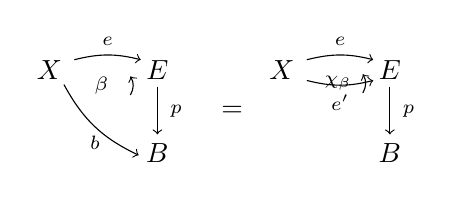
\begin{tikzpicture}[x=1.5em,y=1.5em]
  \begin{scope}[shift={(0,0)}]
  \node (E) at (2.6,1.1) {$E$};
  \node (X) at (0,1.1) {$X$};
  \node (B) at (2.6,-0.9) {$B$};
  \draw[->] (0.6,1.35) to[bend left=14] node[above]{$\scriptstyle e$} (2.2,1.35);
  \draw[->] (2.6,0.7) -- (2.6,-0.45);
  \node at (3.05,0.1) {$\scriptstyle p$};
  \draw[->] (0.35,0.75) to[bend right=18] node[below,pos=0.5]{$\scriptstyle b$} (2.15,-0.95);
  \draw[->] (1.95,0.5) to[bend right=30] (1.95,0.95);
  \node at (1.25,0.72) {$\scriptstyle\beta$};
  \node at (4.4,0.1) {$=$};
  \end{scope}
  \begin{scope}[shift={(5.6,0)}]
  \node (E) at (2.6,1.1) {$E$};
  \node (X) at (0,1.1) {$X$};
  \node (B) at (2.6,-0.9) {$B$};
  \draw[->] (0.6,1.35) to[bend left=14] node[above]{$\scriptstyle e$} (2.2,1.35);
  \draw[->] (0.6,0.85) to[bend right=14] node[below]{$\scriptstyle e'$} (2.2,0.85);
  \draw[->] (2.6,0.7) -- (2.6,-0.45);
  \node at (3.05,0.1) {$\scriptstyle p$};
  \draw[->] (1.95,0.55) to[bend right=30] (1.95,1.0);
  \node at (1.35,0.78) {$\scriptstyle\chi_{\beta}$};
  \end{scope}
\end{tikzpicture}
\end{center}
使得对任何\trFunctor{} $f\colon Y\to X$，2-胞腔 $\chi_{\beta}f$ 在%
\trHomotopyTwoCategory{}中满足下列性质：
\begin{enumerate}[label=(\roman*)]
\item \textbf{归纳：}给定任意 2-胞腔 $\tau\colon e''\Rightarrow ef$ 与
$\gamma\colon pe''\Rightarrow pe'f$，使得 $p\tau=\beta f\cdot\gamma$，则存在
$\gamma$ 的一个\trLifting{} $\bar{\gamma}\colon e''\Rightarrow e'f$，使得
$\tau=\chi_{\beta}f\cdot\bar{\gamma}$。
\item \textbf{保守性：}$\chi_{\beta}f$ 的任何纤维化自同态皆可逆：对任何满足
$\chi_{\beta}f\cdot\zeta=\chi_{\beta}f$ 且 $p\zeta=\mathrm{id}_{pe'f}$ 的 2-胞腔
$\zeta\colon e'f\Rightarrow e'f$，$\zeta$ 可逆。
\end{enumerate}
此外，在这些假设之下，余定义域为 $E$ 的\trNaturalTransformation{}
$\psi\colon e'\Rightarrow e$ 是 $p$-\trCartesian，当且仅当 $\psi$ 在
$f=\mathrm{id}$ 的情形下满足归纳与保守性条件。
\end{proposition}

为在证明中保持条理，我们把满足条件 (i) 与 (ii) 的\trNaturalTransformation{}
$\psi\colon e'\Rightarrow e$ 称作\emph{弱 $p$-笛卡尔变换}。我们将论证：当 $p$
是\trCartesianFibration{}时，弱 $p$-笛卡尔变换类与 $p$-笛卡尔变换类相重合。

\begin{proof}
若 $p\colon E\twoheadrightarrow B$ 是\trCartesianFibration，则任何
$\beta\colon b\Rightarrow pe$ 都容有一个 $p$-笛卡尔提升
$\chi_{\beta}\colon\beta^{*}e\Rightarrow e$。由引理 5.1.4，沿任何函子的限制
$\chi_{\beta}f$ 仍是 $p$-笛卡尔变换。由命题 5.1.13，这个 $\chi_{\beta}f$ 便满足
归纳与保守性性质。事实上，命题 5.1.13 更一般地表明：任何 $p$-笛卡尔变换都是弱
$p$-\trCartesian。

反之，设 $p\colon E\twoheadrightarrow B$ 满足题设。我们将利用与 $p$ 之上的右
逗号锥 $\phi$ 的提升
\begin{center}
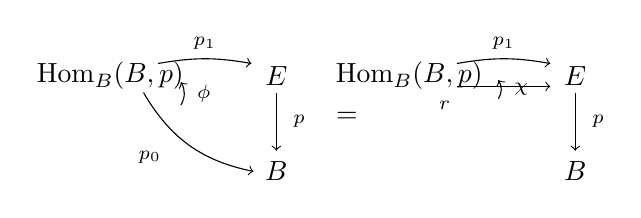
\begin{tikzpicture}[x=1.5em,y=1.5em]
  \begin{scope}[shift={(0,0)}]
  \node (H) at (0,1.1) {$\mathrm{Hom}_{B}(B,p)$};
  \node (E) at (4.0,1.1) {$E$};
  \node (B) at (4.0,-1.2) {$B$};
  \draw[->] (1.15,1.4) to[bend left=10] node[above]{$\scriptstyle p_{1}$} (3.4,1.4);
  \draw[->] (4.0,0.7) -- (4.0,-0.7);
  \node at (4.55,0) {$\scriptstyle p$};
  \draw[->] (0.8,0.7) to[bend right=24] (3.45,-1.2);
  \node at (0.95,-0.85) {$\scriptstyle p_{0}$};
  \draw[->] (1.7,0.4) to[bend right=30] (1.7,0.95);
  \node at (2.25,0.68) {$\scriptstyle\phi$};
  \node at (5.7,0.1) {$=$};
  \end{scope}
  \begin{scope}[shift={(7.2,0)}]
  \node (H) at (0,1.1) {$\mathrm{Hom}_{B}(B,p)$};
  \node (E) at (4.0,1.1) {$E$};
  \node (B) at (4.0,-1.2) {$B$};
  \draw[->] (1.15,1.4) to[bend left=10] node[above]{$\scriptstyle p_{1}$} (3.4,1.4);
  \draw[->] (1.15,0.85) -- (3.4,0.85);
  \node at (0.85,0.4) {$\scriptstyle r$};
  \draw[->] (4.0,0.7) -- (4.0,-0.7);
  \node at (4.55,0) {$\scriptstyle p$};
  \draw[->] (2.15,0.55) to[bend right=30] (2.15,1.0);
  \node at (2.7,0.78) {$\scriptstyle\chi$};
  \end{scope}
\end{tikzpicture}
\end{center}
及其诸限制相关联的归纳与保守性性质，来构造\cref{thm:internal-characterization}(iii)
的数据。

首先，我们把归纳性质应用于 $\chi\Delta_{p}\colon r\Delta_{p}\Rightarrow\mathrm{id}_{E}$，
诱导出一个 2-胞腔 $\eta\colon\mathrm{id}_{E}\Rightarrow r\Delta_{p}$，使得
$p\eta=\mathrm{id}_{p}$ 且 $\chi\Delta_{p}\cdot\eta=\mathrm{id}$。由构造，
$\eta\cdot\chi\Delta_{p}$ 定义了 $\chi\Delta_{p}$ 的一个纤维化自同构，故由保守性
性质必可逆。于是，纤维化 2-胞腔 $\eta$ 是 $\chi\Delta_{p}$ 的逆同构。

我们由 2-胞腔归纳，从 2-胞腔对 $p_{1}\epsilon=\chi$ 与 $p_{0}\epsilon=\mathrm{id}$
诱导出\trCounit{} $\epsilon\colon\Delta_{p}r\Rightarrow\mathrm{id}$。由于
$\epsilon\Delta_{p}$ 由一对可逆 2-胞腔诱导而来，由\trTwoCellConservativity{}它必
是\trIsomorphism。2-胞腔 $r\epsilon$ 也可看出是可逆的，理由是与水平复合相关联的
须化方块的自然性：
\begin{center}
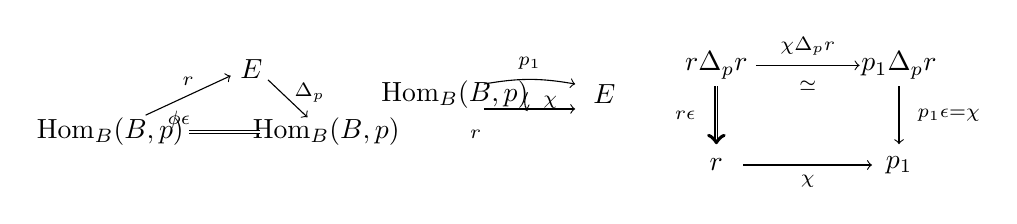
\begin{tikzpicture}[x=1.5em,y=1.5em]
  \begin{scope}[shift={(0,0)}]
  \node (E)  at (3.4,1.5) {$E$};
  \node (H1) at (0,0) {$\mathrm{Hom}_{B}(B,p)$};
  \node (H2) at (5.2,0) {$\mathrm{Hom}_{B}(B,p)$};
  \draw[->] (0.85,0.4) -- node[above,pos=0.5]{$\scriptstyle r$} (2.9,1.35);
  \node at (1.65,0.3) {$\scriptstyle\phi\epsilon$};
  \draw[->] (3.8,1.25) -- (4.75,0.35);
  \node at (4.8,0.95) {$\scriptstyle\Delta_{p}$};
  \draw[double] (1.9,0) -- (3.6,0);
  \end{scope}
  \node at (7.3,0.7) {$\rightsquigarrow$};
  \begin{scope}[shift={(8.3,0)}]
  \node (H) at (0,0.9) {$\mathrm{Hom}_{B}(B,p)$};
  \node (E) at (3.6,0.9) {$E$};
  \draw[->] (0.7,1.15) to[bend left=10] node[above]{$\scriptstyle p_{1}$} (2.9,1.15);
  \draw[->] (0.7,0.55) -- (2.9,0.55);
  \node at (0.5,-0.05) {$\scriptstyle r$};
  \draw[->] (1.75,0.95) to[bend right=30] (1.75,0.5);
  \node at (2.3,0.72) {$\scriptstyle\chi$};
  \end{scope}
  \node at (13.4,0.7) {$\rightsquigarrow$};
  \begin{scope}[shift={(14.6,0)}]
  \node (rdr) at (0,1.6) {$r\Delta_{p}r$};
  \node (pdr) at (4.4,1.6) {$p_{1}\Delta_{p}r$};
  \node (r)   at (0,-0.8) {$r$};
  \node (p1)  at (4.4,-0.8) {$p_{1}$};
  \draw[->] (0.95,1.6) -- node[above]{$\scriptstyle\chi\Delta_{p}r$} (3.45,1.6);
  \node at (2.2,1.12) {$\scriptstyle\simeq$};
  \draw[double,->] (0,1.1) -- (0,-0.3);
  \node at (-0.75,0.4) {$\scriptstyle r\epsilon$};
  \draw[->] (4.4,1.1) -- (4.4,-0.3);
  \node at (5.6,0.4) {$\scriptstyle p_{1}\epsilon=\chi$};
  \draw[->] (0.65,-0.8) -- node[below]{$\scriptstyle\chi$} (3.75,-0.8);
  \end{scope}
\end{tikzpicture}
\end{center}
弱 $p$-笛卡尔胞腔在\trIsomorphism{}下稳定，故右上角的复合是弱 $p$-\trCartesian。
由于 $pr\epsilon=p_{0}\epsilon=\mathrm{id}$，我们可以再次应用归纳与保守性性质，
诱导出一个变换 $\gamma\colon r\Rightarrow r\Delta_{p}r$，使得 $\gamma\cdot r\epsilon$
与 $r\epsilon\cdot\gamma$ 都是\trIsomorphism。于是 $r\epsilon$ 可逆。

由引理 2.1.11，\trInfinityCosmos{} $\mathcal{K}$ 中的这份数据足以在切片%
\trHomotopyTwoCategory{}
$(\hbar\mathcal{K})_{/B}$ 中定义一个伴随。由引理 3.6.7，这个伴随随后可以沿命题
3.6.2 的覆盖 2-函子 $\hbar(\mathcal{K}_{/B})\to(\hbar\mathcal{K})_{/B}$ 提升为一
个真正的\trFiberedAdjunction。由\cref{thm:internal-characterization}(iii)，这就证明了 $p$
是一条\trCartesianFibration。

最后，注意当 $p\colon E\twoheadrightarrow B$ 是\trCartesianFibration{}时，任何
在 $f=\mathrm{id}$ 情形下满足 (i) 与 (ii) 的 $\psi\colon e'\Rightarrow e$ 都与
余定义域为 $e$ 的 $p\psi$ 的某个 $p$-笛卡尔提升成\trFiberedIsomorphism。由引理
5.1.6，由此可知 $\psi$ 便是一条 $p$-笛卡尔变换，这就证明了当 $p$ 是%
\trCartesianFibration{}时这两个类相重合。
\end{proof}


\subsection*{练习}

\begin{exercise}\label{ex:street-cartesian-fibrations}
Street [118] 在 2-范畴中发展了\trCartesianFibration{}的一个标准概念，它在特化到
2-范畴 $\mathcal{C}at$ 时复原出 Grothendieck \trFibration。这并\emph{不是}%
\trInfinityCategory{}之间的\trCartesianFibration{}的正确概念，因为通常概念对被
提升 2-胞腔所要求的\trUniversalProperty{}过于严格。请将此定义与%
\cref{prop:external-characterization}的 2-范畴式定义相比较，并思考为何这个更严格
的\trUniversalProperty{}在\trInfinityCategory{}语境中不成立，例如可以借由考察%
\cref{prop:domain-projection-fibration}的\trCartesianFibration{}来思考。
\end{exercise}

\begin{exercise}\label{ex:incoherent-pseudofunctor}
证明：一条\trCartesianFibration{} $p\colon E\twoheadrightarrow B$ 定义了一个
「不相干拟函子」$E\colon\mathrm{h}B^{\mathrm{op}}\rightsquigarrow\hbar\mathcal{K}$，
由如下数据给出：
\begin{itemize}
\item 对象上的映射 $b\in\mathrm{h}B\mapsto E_{b}\in\hbar\mathcal{K}$；
\item 1-胞腔上的映射 $\beta\colon a\to b\in\mathrm{h}B\mapsto\beta^{*}\colon E_{b}\to E_{a}\in\hbar\mathcal{K}$，由 (5.0.1) 定义；
\item 对每个 $b\in\mathrm{h}B$ 的一个可逆 2-胞腔
\cellpair{E_{b}}{E_{b}}{\mathrm{id}_{E_{b}}}{\mathrm{id}_{b}^{*}}{\iota_{b}}
$\in\hbar\mathcal{K}$；以及
\item 对 $\mathrm{h}B$ 中每对可复合的箭头 $\beta\colon a\to b$ 与
$\gamma\colon b\to c$ 的一个可逆 2-胞腔
\begin{center}
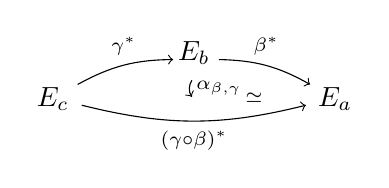
\begin{tikzpicture}[x=1.5em,y=1.5em]
  \node (Ec) at (0,0) {$E_{c}$};
  \node (Eb) at (3.4,1.1) {$E_{b}$};
  \node (Ea) at (6.8,0) {$E_{a}$};
  \draw[->] (0.6,0.35) to[bend left=14] node[above,pos=0.5]{$\scriptstyle\gamma^{*}$} (2.9,0.95);
  \draw[->] (4.0,0.95) to[bend left=14] node[above,pos=0.5]{$\scriptstyle\beta^{*}$} (6.2,0.35);
  \draw[->] (0.7,-0.15) to[bend right=14] node[below]{$\scriptstyle(\gamma\circ\beta)^{*}$} (6.1,-0.15);
  \draw[->] (3.35,0.45) to[bend right=30] (3.35,0.05);
  \node at (4.0,0.25) {$\scriptstyle\alpha_{\beta,\gamma}$};
  \node at (4.85,0.02) {$\scriptstyle\simeq$};
\end{tikzpicture}
\end{center}
$\in\hbar\mathcal{K}$。
\end{itemize}
一个\textbf{拟函子}（pseudo-functor）的完整定义中所出现的诸相容性条件（见定义
10.4.1）在此并不明显，但它们确实可以由把这个构造扩充为以 $B$ 的%
\trUnderlyingQuasiCategory{}为指标的同伦相干图表而得出 [111, 6.1.16]。
\end{exercise}


\begin{exercise}\label{ex:cospan-domain-projection-fibration}
（5.5.13）利用\cref{thm:internal-characterization}的 (iii) 或 (ii) 之任一证明：
对\trInfinityCategory{}之间的任意函子\trCospan{}
$C\xrightarrow{g}A\xleftarrow{f}B$，定义域投影函子
$p_{0}\colon\mathrm{Hom}_{A}(f,g)\twoheadrightarrow B$ 是一条%
\trCartesianFibration，此外，余定义域为 $\mathrm{Hom}_{A}(f,g)$ 的%
\trNaturalTransformation{} $\psi$ 是 $p_{0}$-\trCartesian，当且仅当
$p_{1}\psi$ 可逆。\footnote{由\cref{prop:pullback-stability}与如下拉回方块
\begin{center}
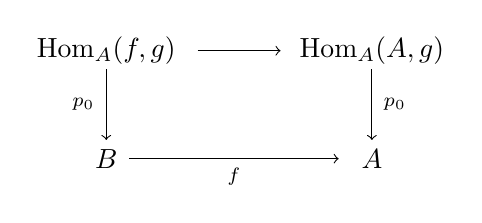
\begin{tikzpicture}[x=1.5em,y=1.5em]
  \node (fg) at (0,1.3) {$\mathrm{Hom}_{A}(f,g)$};
  \node (Ag) at (6.4,1.3) {$\mathrm{Hom}_{A}(A,g)$};
  \node (B)  at (0,-1.3) {$B$};
  \node (A)  at (6.4,-1.3) {$A$};
  \draw[->] (2.2,1.3) -- (4.2,1.3);
  \draw[->] (0,0.85) -- (0,-0.85);  \node at (-0.55,0) {$\scriptstyle p_{0}$};
  \draw[->] (6.4,0.85) -- (6.4,-0.85);  \node at (6.95,0) {$\scriptstyle p_{0}$};
  \draw[->] (0.55,-1.3) -- node[below]{$\scriptstyle f$} (5.6,-1.3);
  \node at (0.5,0.82) {$\scriptstyle\llcorner$};
\end{tikzpicture}
\end{center}
只需证明定义域投影函子 $p_{0}\colon\mathrm{Hom}_{A}(A,g)\twoheadrightarrow A$
是一条\trCartesianFibration{}即可。在某种意义上，这个函子可以理解为
$p_{0}\colon A^{2}\twoheadrightarrow A$ 的一个拉回，我们将在推论 5.5.13 的
证明中解释这一点——该结果即出现于彼处。如果这一构造实在过于痛苦，有意重演%
\cref{prop:domain-projection-fibration}之证明的读者不妨转而求助于命题 6.3.10。}
\end{exercise}


